%
%   CHAPTER : THEORETICAL BACKGROUND FOR EXPERIMENTS AND EVALUATION
%   
%   Wichtige Punkte : 
%    + Ramanstreuung, projektbericht anreißen (-> was bedeutet tensor? was ist depolarisationsgrad?)
%    + Kurz: Herkunft Raman-Müller-Matrix; Genauigkeitsprobleme durch iterative Monte-Carlo-Simulation
%    + Müllerformalismus/-matrix (Was machen verwendete Bauteile? Wie machen die das? Bezug zu ihrer Müllermatrix)
%    + Aufbau Ramanspektrometer; Welche Teile sind polarisationsempfindlich? -> Warum glauben wir Polarisation kann das Ergebnis beeinflussen
%    + Wie funktionieren optische Faser? Aufbau optische Faser.
%
\documentclass[a4paper,12pt,twoside,parskip=no,headsepline,open=right,ngerman,export]{scrreprt}

%
%   Include shared preamble
%   Preamble is put into seperate file to be used in files included with \input
%   Made possible with standalone package
%
%
%   PREAMBLE SHARED BY MASTER FILE AND ALL SUBFILES
%
%
%   USED PACKAGES AND STYLES
%

%
%   KEINE AHNUNG; IST KRAM DEN JULIAN IN SEINEM TEMPLATE HATTE
%
\usepackage{newunicodechar}
\usepackage{comment}
%\usepackage{acro} %Abkürzungen
\usepackage{xcolor} %Farben
\usepackage{rotating}
\usepackage{lmodern}
%\usepackage{parskip}
%\usepackage[crop=off]{auto-pst-pdf} %Einbinden von .eps-Dateien in PDFTeX
\usepackage{paralist}

%
%   UTILITIES
%
%\usepackage{hyperref}

%
%   LANGUAGE, FONT
%
\usepackage[utf8]{inputenc} % Eingabe-Codierung
\usepackage[ngerman]{babel} % Spracheinstellung
\usepackage[T1]{fontenc}    % Anpassung auf europäischen Zeichensatz
\usepackage{xspace}         % Leerzeichen für Silbentrennung
\usepackage{hyphenat}       % Korrekte Silbentrennung


%
%   MULTIPLE FILES
%
\usepackage{pdfpages}   % Include pdf files
\usepackage{standalone} % Include .tex/.Rtex documents that have their own preamble and \begin{documents}

%
%   INHALTSVERZEICHNIS UND ÄHNLICHES
%
%%Umbennenung Inhaltsverzeichnis
\addto\captionsenglish{%
\renewcommand{\contentsname}{Inhaltsverzeichnis}}

%
%   FIGURES AND TABLES
%
\usepackage{subfig}                     % Mutli image figures
\usepackage[format=plain]{caption} %Einstellen der caption-Breite
\captionsetup[table]{skip=10pt}
\usepackage{wrapfig} %Floats von Text umflossen
\usepackage{float} %Position von figure/table erzwingen
\usepackage{flafter} %Floats nach Definition!
\usepackage{graphicx}
\usepackage{booktabs}
\usepackage{multicol}
\usepackage{multirow}


%
%   LITERATUR
%
\usepackage[style=chem-angew,
            doi=true,
			sorting=none,
			backend=biber,
			autocite=superscript,    % Zitate
			minbibnames=3,
			maxbibnames=5
			]{biblatex}
\usepackage{csquotes}                % Formattieren von Zitaten (Anfürhungszeichen)


%
%   MATHEMATIK
%
\usepackage{amsmath} %mathematischer Satz
\usepackage{amsfonts} %mathematische Schriftart
\usepackage{amssymb} %mathematische Symbole
\usepackage[output-decimal-marker={,},
            group-separator = {.}, 
            group-digits=true,
            detect-weight]{siunitx}     % korrekte Formatierung von Einheiten nach SI-Kriterien
\usepackage{nicefrac}
\usepackage{mathtools}  % pmatrix* environment for aligning matrix elements

%
%   CHEMIE
%
%\usepackage{chemgreek}
%\usepackage{chemnum} %Nummerierung der Verbindung aus ChemDraw
\usepackage[version=4]{mhchem} %Darstellung von chemischen Formeln
\usepackage{chemmacros}         % Abkürzungen (pH, pKa, ...) und Ladungen

%
%   FORMATTING, PAGE STYLE
%
\usepackage{setspace} %Zeilenabstand
%\usepackage{titlesec} %Verändern von Überschrift-Formatierungen
\usepackage[headsepline]{scrlayer-scrpage}

%
% INCLUDE SOURCE CODE
%
\definecolor{dkgreen}{rgb}{0,0.6,0}
\definecolor{gray}{rgb}{0.5,0.5,0.5}
\definecolor{mauve}{rgb}{0.58,0,0.82}
\usepackage{listings} %Programmiersprachen einbinden
\lstloadlanguages{R}
\lstset{frame=tb,
  language=R,
  aboveskip=3mm,
  belowskip=3mm,
  showstringspaces=false,
  columns=flexible,
  basicstyle={\small\ttfamily},
  numbers=none,
  numberstyle=\tiny\color{gray},
  keywordstyle=\color{blue},
  commentstyle=\color{dkgreen},
  stringstyle=\color{mauve},
  breaklines=true,
  breakatwhitespace=true,
  tabsize=4
}



%
%   JULIANS TEMPLATE COMMANDS
%   KEINE AHNUNG WAS ER DA GEMACHT HAT
%
\newcommand{\ts}{\textsubscript} %tiefstellen
\newcommand{\te}{\textsuperscript} %hochstellen
\newcommand{\grad}{\degreeCelsius}


%\setlength{\parindent}{0pt}


\setcounter{secnumdepth}{4}

\DeclareUnicodeCharacter{00A0}{ }

\newlength\myheight

\newlength\mywidth



\clubpenalty10000
\widowpenalty10000
\displaywidowpenalty=10000

%\raggedbottom

%\renewcommand{\lstlistingname}{Code}

\floatstyle{plaintop}
\newfloat{code}{tbp}{lop}[chapter]
\floatname{code}{Code}
%
%   ENDE JULIANS TEMPLATE
%	
%
%   SOME CUSTOM COMMANDS AND SHORTCUTS
%

% MATHEMATICS AND FORMULAS
\newcommand{\ring}[1]{\text{\r{#1}}}	    % Shortcut for writing circle above character
\newcommand{\vc}[1]{\vec{#1}}               % Shortcut for uniformly formatting vectors
\newcommand{\mx}[1]{\boldsymbol#1}          % Shrotcut for uniformly formatting matrices
\newcommand{\tildenu}{\tilde{\nu}}          % Shortcut for wave number symbol

% FORMATTING
\newcommand{\optelem}[1]{\textbf{#1}}       % Shortcut for uniforly formate optical elements
\newcommand{\chemical}[1]{\textbf{#1}}      % Shortcut for uniforly formate chemical abreviations

% REMINDERS
\def\quelle{~\textbf{[QUELLE]}}

% -----------------------------------------
% Makros used to make integral sign match matrix/fraction height
%
\def\tmp#1 #2\relax{#1}
\setbox0=\hbox{$\xdef\intfont{%
    \expandafter\tmp\fontname\textfont3\expandafter\space\space\relax}$}
\font\tmp=\intfont\space at10pt\relax
\setbox0=\hbox{$\textfont3=\tmp \displaystyle \int$}
\dimen0=\ht0 \advance\dimen0 by\dp0 \divide\dimen0 by10 
\xdef\intsize{\the\dimen0}

\def\dividedimen (#1/#2){\expandafter\ignorept\the
   \dimexpr\numexpr\number\dimexpr#1\relax
   *65536/\number\dimexpr#2\relax\relax sp\relax
}
{\lccode`\?=`\p \lccode`\!=`\t  \lowercase{\gdef\ignorept#1?!{#1}}}
% Makros used to make integral sign match matrix/fraction height
\def\flexibleint{\def\fxintL{}\def\fxintU{}\futurelet\next\fxintA}
\def\fxintA{\ifx\next_\expandafter\fxintB\else\expandafter\fxintC\fi}
\def\fxintB_#1{\def\fxintL{#1}\fxintC}
\def\fxintC{\futurelet\next\fxintD}
\def\fxintD{\ifx\next^\expandafter\fxintE\else\expandafter\fxintF\fi}
\def\fxintE^#1{\def\fxintU{#1}\fxintF}
\def\fxintF#1{\begingroup
   \setbox0=\hbox{$\displaystyle{#1}$}%
   \dimen0=\ht0 \advance\dimen0 by\dp0
   \setbox1=\hbox{$\vcenter{\copy0}$}%
   \font\tmp=\intfont\space at\dividedimen(\dimen0/\intsize)pt
   \lower\dimexpr\dp0-\dp1\hbox{%
      $\textfont3=\tmp \displaystyle\int_{\fxintL}^{\fxintU}$}
   \box0
   \endgroup
}
%
% END: makros for making integral match fraction/matrix height
% --------------------------------------------
%\input{./sup/abreviations.tex}
%
%   CUSTOM HYPHENATION
%

%\hyphenation{Kor-re-la-ti-ons-spek-tro-sko-pie Kor-re-la-ti-ons-spek-trum Spek-tro-sko-pie}
\hyphenation{Stan-dard-ab-wei-chung}
\hyphenation{Halb-wel-len-plat-te Halb-wel-len-plat-ten}
\hyphenation{Ra-man-Mül-ler-trans-for-ma-tion}
\hyphenation{An-ti-Sto-kes-Ver-schie-bung}
\hyphenation{Sto-kes-Ver-schie-bung}


%
%   LITERATUR
%
\addbibresource{./sup/lit.bib}	
\AtEveryBibitem{\clearfield{note}}    % clears notes

%
%   SEITENEINSTELLUNG
%
%Druckbereich wählen (\areaset[BCOR]{breite}{höhe})
\areaset[13 mm]{140mm}{250mm}
\pagestyle{scrheadings}


%
%   KOPFZEILE
%
\chead{\leftmark}
\ihead{}
\ohead{}
\ofoot{\thepage}
\automark{chapter}


%
%   SEITENSTIL
%
\setstretch{1.15} %Zeilenabstand einstellen
\pagenumbering{arabic}
\setcounter{page}{1}

%
%   DOCUMENT
%
\begin{document}

    \chapter{Einführung}
        
        %
        %   RAMANSTREUUNG
        %
        \section{Ramanstreuung von elektromagnetischen Wellen}
            
            Die Interaktion von elektromagnetischen Wellen mit Materie lässt sich über induzierte Dipole beschreiben. Das elektrische Feld der Welle $\vc{E}(t) = \vc{E}_0 \cos(2\pi \nu t)$ oszilliert mit einer Frequenz von $\nu$ und induziert einen in Phase schwingenden Dipol $\vc{\mu}(t) = \vc{\mu}_0 \cos(2\pi \nu t)$~\cite{chalmers_raman_2006}. Dieser Hertzsche Dipol erzeugt selbst elektromagnetische Wellen mit der Frequenz $\nu$, die sich in viele Raumrichtungen ausbreiten: Das Licht wird gestreut. Die Intensität der Streustrahlung ist proportional zur der Amplitude des Dipols und hängt von der Amplitude des anregenden Feldes $|\vc{E}|$ und der Polarisierbarkeit $\mx{\alpha}$ des Moleküls ab~\cite{wilson_molecular_1955}.
            \begin{equation}
                \begin{pmatrix} \mu_x \\ \mu_y \\ \mu_z \end{pmatrix} 
                    = \mx{\alpha} \cdot \begin{pmatrix} E_x \\ E_y \\ E_z \end{pmatrix}
                \label{eq:theo_rayleighDipol}
            \end{equation}
            Da Moleküle nicht kugelsymmetrisch sind, hängt die Polarisierbarkeit des Moleküls seiner der Orientierung zum anregenden elektrischen Feld ab. Die anisotrope Polarisierbarkeit wird als $3\times 3$-Tensor $\mx{\alpha}$ dargestellt~\cite{chalmers_raman_2006}. Dieser Tensor kann durch Multiplikation mit Rotationsmatrizen in beliebige Molekülorientierungen überführt werden.
            
            Die Polarisierbarkeit wird neben der Molekülstruktur auch durch die Schwingung des Moleküls beeinflusst. Zum Beispiel erhöht sich durch Stauchung einer Bindung die lokale Ladungsdichte: Die Polarisierbarkeit sinkt~\cite{chalmers_raman_2006}. Wird der Polarisierbarkeitstensor in seiner diagonalisierten Form 
            \begin{equation}
                \mx{\alpha} = \begin{pmatrix}   \alpha_x  & 0         & 0 \\
                                                0         & \alpha_y  & 0 \\
                                                0         & 0         & \alpha_z
                              \end{pmatrix}
            \end{equation}
            betrachtet, beschreibt Gleichung~\ref{eq:theo_polarisierbarkeitTaylor} im Rahmen einer linearen Näherung die schwingungsbedingte Zeitabhängigkeit des $i$-ten Tensorelements~\cite{wilson_molecular_1955}.
            \begin{equation}
                \alpha_i(t) \approx \alpha_{0,i} + \sum_k \left(\frac{\partial \alpha_i}{\partial Q_k}\right)_0 \cdot Q_k(t)
                \label{eq:theo_polarisierbarkeitTaylor}
            \end{equation}
            Die Schwingung des Moleküls wird durch seine Normalmoden dargestellt. Die $k$-te Normalmode $Q_k(t) = Q_{0,k} \cos(2\pi \nu_k t)$ schwingt dabei mit der Amplitude $Q_{0,k}$ und der Frequenz $\nu_k$. Die zeitabhängige Polarisierbarkeit $\alpha_i(t)$ setzt sich aus zwei Komponenten zusammen: Die Polarisierbarkeit in der Gleichgewichtslage der Molekülschwingung $\alpha_{0,i}$ und die Änderung der Polarisierbarkeit für die $k$-te Normalmode in der Nähe der Gleichgewichtslage $(\nicefrac{\partial \alpha_i}{\partial Q_k})_0$~\cite{wilson_molecular_1955}.
            
            Wird in Gleichung~\ref{eq:theo_rayleighDipol} die Zeitabhängigkeit der Polarisierbarkeit berücksichtigt, lässt sich der Ramanstreuprozess beschreiben. Dafür wird Gleichung~\ref{eq:theo_polarisierbarkeitTaylor} in Gleichung~\ref{eq:theo_rayleighDipol} eingesetzt~\cite{wilson_molecular_1955}.
            \begin{align*}
                \mu_i(t) &= \alpha_i \cdot E_i(t) \\
                \mu_i(t) &= 
                    \left[  \alpha_{0,i} 
                        + \sum_k \left(\frac{\partial \alpha_i}{\partial Q_k}\right)_0 \cdot Q_k(t) 
                    \right] \cdot E_i(t)
            \end{align*}
            Mit $Q_k(t) = Q_{0,k} \cos(2\pi \nu_k t)$ und $E_i = E_{0,i}\cos(2\pi \nu t)$.
            \begin{align*}
                \mu_i(t) &= \left[  \alpha_{0,i} 
                        + \sum_k \left(\frac{\partial \alpha_i}{\partial Q_k}\right)_0 
                          \cdot Q_{0,k} \cos(2\pi \nu_k t) 
                    \right] \cdot E_{0,i}\cos(2\pi \nu t) \\
                \mu_i(t) &= \alpha_{0,i} \cdot E_{0,i}\cos(2\pi \nu t)
                        + \sum_k \left(\frac{\partial \alpha_i}{\partial Q_k}\right)_0 
                          \cdot Q_{0,k} \cdot E_{0,i} \cos(2\pi \nu_k t) \cdot \cos(2\pi \nu t)
            \end{align*}
            Mit $\cos(a x)\cdot\cos(b x) = \frac{1}{2}\cos[(a+b)x] +\frac{1}{2}\cos[(a-b)x]$~\cite{bronstein_taschenbuch_2000}.
            \begin{equation}
                \begin{array}{r rc cc c}
                    \mu_i(t) =& E_{0,i} &\cdot& \alpha_{0,i}                                                   &\cdot& \cos(2\pi \nu t) \\
                    +&\sum_k    E_{0,i} &\cdot& \left(\frac{\partial \alpha_i}{\partial Q_k}\right)_0 Q_{0,k}  &\cdot& \frac{1}{2} \cos[2\pi (\nu+\nu_k) t] \\
                    +&\sum_k    E_{0,i} &\cdot& \left(\frac{\partial \alpha_i}{\partial Q_k}\right)_0 Q_{0,k}  &\cdot& \frac{1}{2}\cos[2\pi (\nu-\nu_k) t]
                \end{array}
                \label{eq:theo_ramanDipol}
            \end{equation}
            Gleichung~\ref{eq:theo_ramanDipol} zeigt, dass mehrere Dipole induziert werden, die mit unterschiedlichen Frequenzen schwingen. 
            
            Es wird ein Dipol induziert, der mit der Anregungsfrequenz $\nu$ schwingt und von der Polarisierbarkeit des Moleküls $\alpha_{0,i}$ abhängt. Dies entspricht der elastischen Streuung an einem nicht schwingenden Molekül nach Gleichung~\ref{eq:theo_rayleighDipol} und wird als Rayleighstreuung bezeichnet.~\cite{chalmers_raman_2006}
            
            Zwei weitere Dipole werden für jede Normalmode $Q_k$ induziert. Diese schwingen mit $\nu\pm\nu_k$ und hängen von der Änderung der Polarisierbarkeit $\left(\nicefrac{\partial \alpha_i}{\partial Q_k}\right)_0 Q_{0,k}$ ab. Dieser inelastische Streuprozess ist der Ramaneffekt. Er erzeugt ein molekülspezifisches Schwingungsspektrum, indem der induzierte Dipol durch die Molekülschwingungen moduliert wird. Das Spektrum tritt sowohl bei größeren 
            $\tildenu+\tildenu_k$ (Stokes\hyp{}Verschiebung) als auch kleineren Wellenzahlen $\tildenu-\tildenu_k$ (Anit\hyp{}Stokes\hyp{}Verschiebung) auf.~\cite{chalmers_raman_2006, wilson_molecular_1955}

            Wie bei der Rayleighstreuung wird jede Mode $Q_k$ durch ihren eigenen Tensor $\mx{\alpha^\prime_k}$ beschrieben. Der Ramantensor der Schwingung $k$
            \begin{equation}
                \mx{\alpha^\prime_k} = \left( \frac{\partial \alpha}{\partial Q_k} \right)_0
            \end{equation}
            ist die Ableitung des Polarisierbarkeitstensors $\mx{\alpha}$ nach der Normalmode $Q_k$ in ihrer Gleichgewichtslage~\cite{chalmers_raman_2006}. 
            
            Dadurch ist auch der Ramantensor im Allgemeinen anisotrop, sodass die Orientierung des Moleküls und auch die Polarisation der elektromagnetischen Welle den Streuprozess beeinflussen~\cite{chalmers_raman_2006}.
            
        %
        %   POLARISATION
        %
        \section{Polarisation im Ramanstreuprozess}\label{sec:theo_raman_mueller}
            
            %
            %   POLARISATION
            %
            \begin{figure}[!b]
                \centering
                \subfloat[]{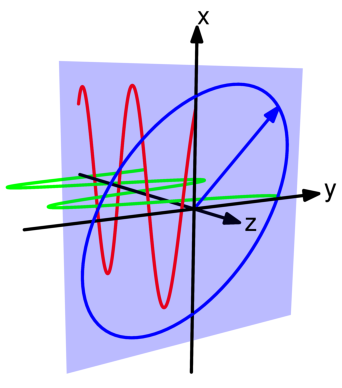
\includegraphics[width=0.33\textwidth]{img/polarisationEllipse}\label{subfig:theo_polarisation_ellipse}} \hfil
                \subfloat[]{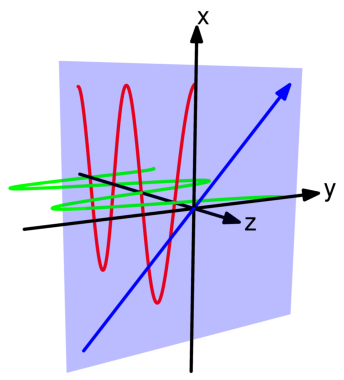
\includegraphics[width=0.33\textwidth]{img/polarisationLinear}\label{subfig:theo_polarisation_linear}} \hfil
                \subfloat[]{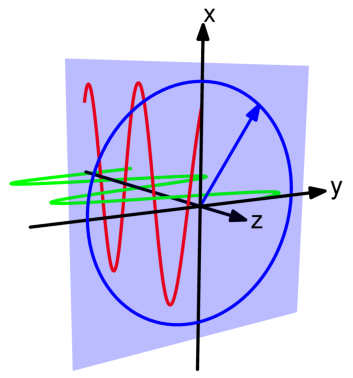
\includegraphics[width=0.33\textwidth]{img/polarisationZirkular}\label{subfig:theo_polarisation_zirkular}}
                \caption[Polarisationsellipse]{Polarisationsarten elektromagnetischer Wellen: Elliptisch \subref{subfig:theo_polarisation_ellipse}, linear \subref{subfig:theo_polarisation_linear} und zirkular polarisiert \subref{subfig:theo_polarisation_zirkular}. Rot und grün zeigen die Oszillation orthogonalen Komponenten des schwingenden elektrischen Feldes. Der elektrische Feldvektor wird in blau dargestellt. Der elektrische Feldvektor (blau) oszilliert mit der Zeit und folgt dabei der blauen Kurve.}
                \label{fig:theo_polarisation}
            \end{figure}
            Elektromagnetische Wellen schwingen transversal~\cite{gil_polarized_2016}. Deshalb können die elektrische Feldvektoren von zwei Wellen mit der gleichen Ausbreitungsrichtung in unterschiedlichen Richtungen oszillieren. Diese Eigenschaft wird durch die Polarisation der Welle beschrieben~\cite{gil_polarized_2016}. Abbildung~\ref{fig:theo_polarisation} zeigt wie Polarisationszustände durch zwei orthogonale elektrische Felder beschrieben werden können. Im allgemeinen Fall sind die schwingenden Felder phasenverschoben und die Strahlung ist elliptisch polarisiert \subref{subfig:theo_polarisation_ellipse}: Die Summe der Felder rotiert mit der Zeit und folgt dabei einer elliptischen Bahn~\cite{gil_polarized_2016}. Die Größe der Phasenverschiebung entscheidet über Exzentrizität und Rotationsrichtung; das Amplitudenverhältnis der elektrischen Felder über den Winkel zwischen großer Halbachse und Abszisse~\cite{gil_polarized_2016}. Ist die Phasenverschiebung gleich einem Viertel der Periode, handelt es sich um den Grenzfall der zirkularen Polarisation~\subref{subfig:theo_polarisation_zirkular}~\cite{gil_polarized_2016}. Der andere Grenzfall tritt für in Phase schwingende Felder auf: die lineare Polarisation~\subref{subfig:theo_polarisation_linear}~\cite{gil_polarized_2016}. Der Feldvektor von linear polarisiertem Licht rotiert nicht, sondern schwingt in einer Ebene orthogonal zur Ausbreitungsrichtung~\cite{gil_polarized_2016}.
            
            %
            %   RAMAN, DEPOLARISATIONSGRAD
            %

            \begin{figure}[!b]
                \centering
                \subfloat[]{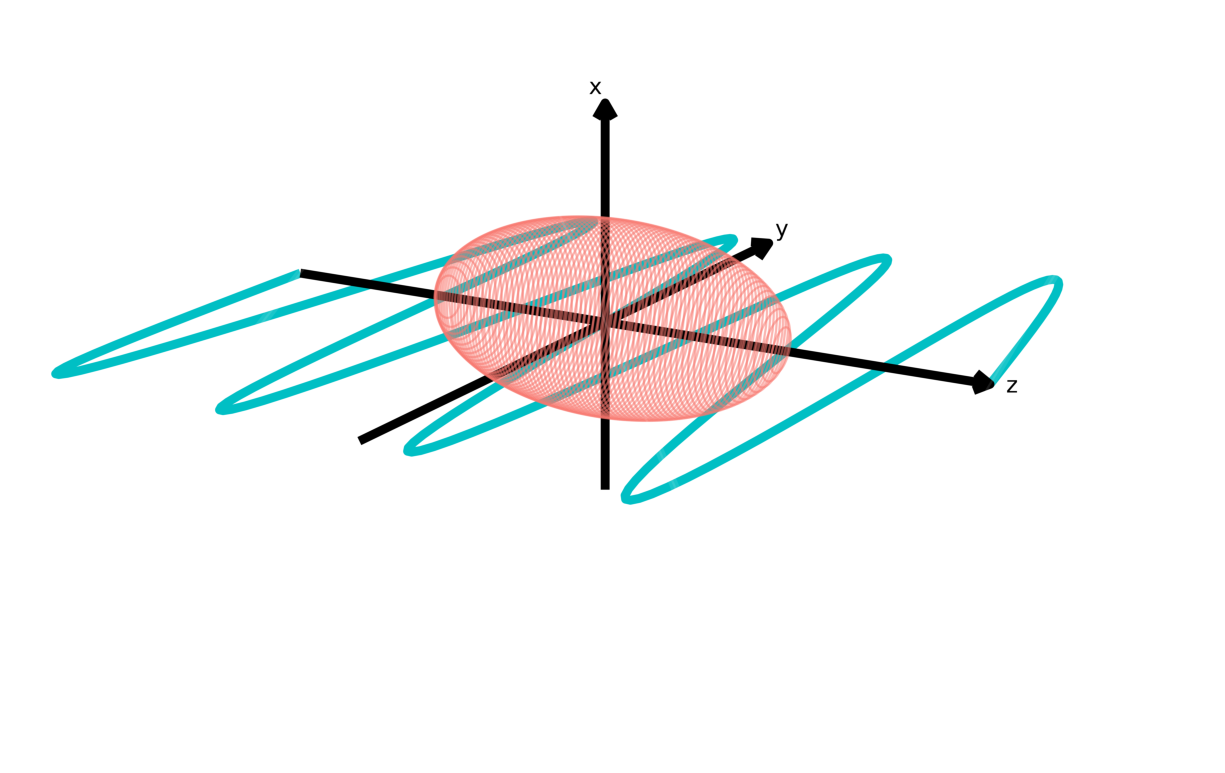
\includegraphics[width=0.5\textwidth]{img/ramanTensor_0deg.pdf}\label{subfig:theo_ramanTensor_0deg}}
                \subfloat[]{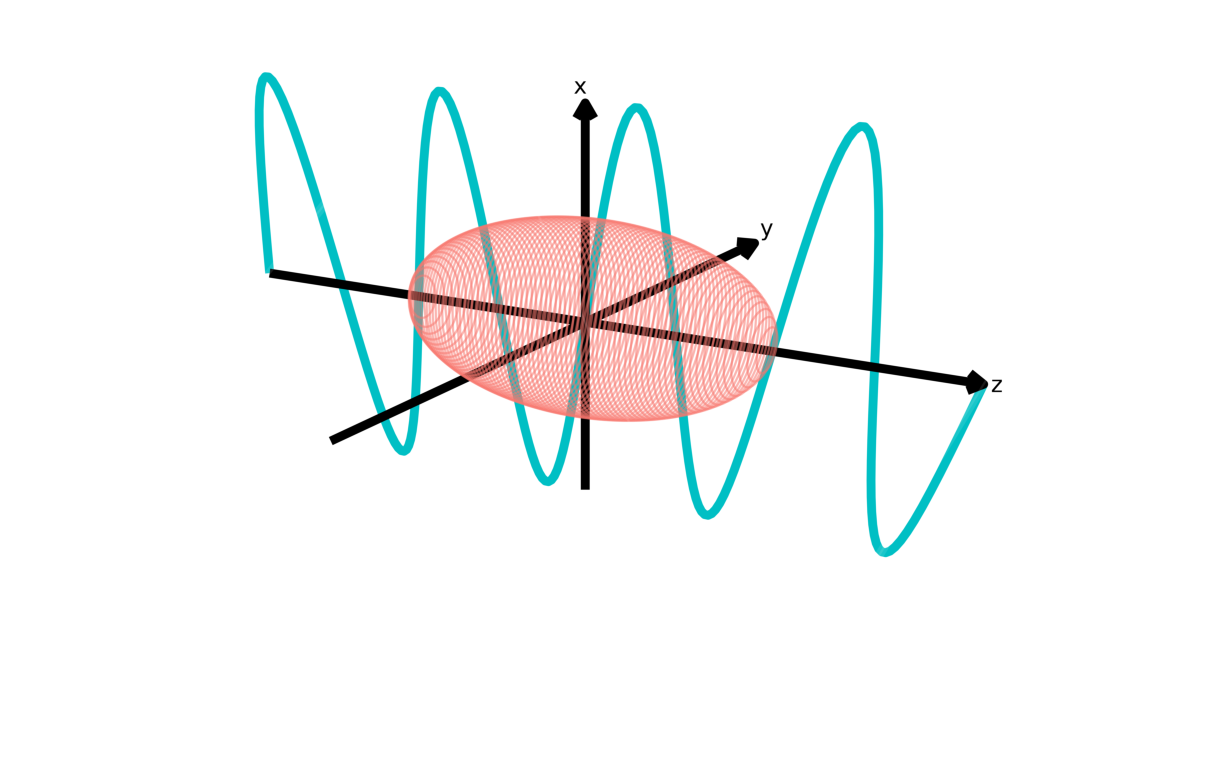
\includegraphics[width=0.5\textwidth]{img/ramanTensor_90deg.pdf}\label{subfig:theo_ramanTensor_90deg}}
                \caption[Polarisationsabhängigkeit der Polarisierbarkeit]{Der rote Ellipsoid demonstriert die räumliche Abhängigkeit der Polarisierbarkeit eines Moleküls. Die Änderung der Polarisationsebene des elektrischen Feldes (blau) von \SI{0}{\degree} \subref{subfig:theo_ramanTensor_0deg} nach \SI{90}{\degree} \subref{subfig:theo_ramanTensor_90deg} hat den gleichen Effekt auf den induzierten Dipol wie die Rotation des Moleküls.}
                \label{fig:theo_ramanTensor}
            \end{figure}
            
            Im vorherigen Abschnitt wurde bereits dargelegt, dass die Orientierung des Moleküls den Streuprozess beeinflusst~\cite{chalmers_raman_2006}. Abbildung~\ref{fig:theo_ramanTensor} illustriert, dass die Orientierung der Polarisationsebene einer linear polarisierten anregenden Welle denselben Effekt hat wie eine Molekülrotation. Um den Einfluss der Streuung auf die Polarisation der Streustrahlung bei frei rotierbaren Systemen makroskopisch zu quantifizieren wird üblicherweise der Depolarisationsgrad $\rho$ verwendet. Wird die Probe mit linear polarisierter Strahlung angeregt, ist der Depolarisationsgrad 
            \begin{equation}
                \rho = \frac{I_{\perp}}{I_{\parallel}} \label{eq:theo_depolarisationRatio_exp}
            \end{equation}
            das Verhältnis der Intensität der Strahlung $I_\parallel$, die parallel, und der Strahlung $I_\perp$, die orthogonal zur ursprünglichen Polarisationsebene ausgerichtet ist~\cite{zare_angular_1988}. Weil der Depolarisationsgrad ein makroskopische Stoffeigenschaft ist, wird sie nicht durch den molekularen Streutensor $\mx{\alpha^\prime}$ beschrieben. Analytisch wird der Depolarisationsgrad ausgehend von einem Streutensor der Form 
            \begin{equation*}
                \mx{\alpha^\prime} = \begin{pmatrix}   \alpha^\prime_x  & 0         & 0 \\
                                                0         & \alpha^\prime_y  & 0 \\
                                                0         & 0         & \alpha^\prime_z
                              \end{pmatrix}
            \end{equation*}
            gemittelt über alle Raumrichtungen bestimmt. Gleichung~\ref{eq:theo_depolarisationRatio_analytic} verknüpft den molekularen Streutensor mit dem makroskopischen Depolarisationsgrad der Schwingung~\cite{zare_angular_1988}.
            \begin{gather}
                \rho = \frac{3 \gamma^2}{45 a^2 + 4 \gamma^2} \label{eq:theo_depolarisationRatio_analytic}\\
                \nonumber
                a = \frac{\alpha^\prime_x + \alpha^\prime_y +\alpha^\prime_z }{3} \\
                \nonumber
                \gamma^2 = \frac{ (\alpha^\prime_x - \alpha^\prime_y)^2 + (\alpha^\prime_y - \alpha^\prime_z)^2 + (\alpha^\prime_z - \alpha^\prime_x)^2 }{2}
            \end{gather}
            Der Depolarisationsgrad nimmt Werte im Interval $[0;\nicefrac{3}{4}]$ an. Die Streuung an einer Probe kann folglich nur maximal \SI{75}{\percent} der Polarisation erhalten. Eine vollständige Depolarisation der Strahlung kann für ausgewählte Molekülschwingungen auftreten~\cite{chalmers_raman_2006}.
            
            %
            %   MUELLER, STOKES
            %
            Unpolarisiertes und partiell polarisiertes Licht lässt sich mit elektrischen Feldern nur schwer beschreiben. Eine einfache Möglichkeit beliebige Polarisationszustände zu diskutieren ist der Müllerformalismus. Der Polarisationszustand wird als vierdimensionaler Stokesvektor
            \begin{equation}
                \vc{S} = \begin{pmatrix} S_0 \\ S_1 \\ S_2 \\ S_3 \end{pmatrix} = \begin{pmatrix} I_x + I_y \\ I_x - I_y \\ I_{x^\prime} - I_{y^\prime} \\ I_{RZ} - I_{LZ} \end{pmatrix}
                \label{eq:theo_stokesVek}
            \end{equation}
            dargestellt und jede Licht-Materie-Wechselwirkung als Matrixmultiplikation $\mx{M}\cdot\vc{S}$ mit einer $4\times 4$-Matrix, welche die polarisierenden und depolarisierenden Eigenschaften der Materie beschreibt.~\cite{gil_polarized_2016}. 
            
            Der erste Stokesvektor $S_0$ beschreibt die Intensität der Strahlung. Häufig werden Stokesvektoren auf $S_0$ normiert~\cite{gil_polarized_2016}; was ein Ersetzen der Intensität durch die experimentell einfacher zugängliche Leistung ermöglicht. Der zweite Stokesparameter $S_1$ beschreibt den Anteil der Strahlung, der entlang der kartesischen Achsen $x$ und $y$ linear polarisiert ist. Ist $S_1 > 0$ überwiegt der Anteil des elektrischen Feldes parallel zur x-Achse, für $S_1 < 0$ überwiegt der Anteil parallel zur y-Achse~\cite{gil_polarized_2016}. Der dritte Stokesparameter $S_2$ ist ein Maß für den Anteil der Strahlung, die entlang der beiden Winkelhalbierenden von $x$- und $y$-Achse linear polarisiert sind. Für $S_2 > 0$ schwingt das elektrische Feld im ersten und dritten Quadranten entlang der $x^\prime$-Achse und für $S_2 < 0$ im zweiten und vierten Quadranten entlang der $y^\prime$-Achse~\cite{gil_polarized_2016}. Der vierte Stokesparameter $S_3$ beschreibt den zirkular polarisierten Teil der Strahlung. $S_3 > 0$ bedeutet, das Licht ist rechts zirkular polarisiert ($RZ$), und $S_3 < 0$, es ist links zirkular polarisiert ($LZ$)~\cite{gil_polarized_2016}. 
            
            Das Verhältnis von $S_1$ und $S_2$ definiert die Lage der Polarisationsebene und das Verhältnis von $S_1$ und $S_2$ zu $S_3$ die Exzentrizität der Polarisationsellipse. Der Polarisationsgrad
            \begin{equation}
                \Pi = \frac{ \sqrt{S_1^2 + S_2^2 + S_3^2} }{S_0}
            \end{equation}
            nimmt Werte zwischen \numlist{0;1} an und beschreibt für $\Pi = 1$ vollständig polarisiertes Licht~\cite{gil_polarized_2016}. Bei $\Pi = 0$ sind die elektrischen Feldkomponenten des Lichts nicht miteinander korreliert und die elektromagnetische Welle ist unpolarisiert~\cite{gil_polarized_2016}. Partiell polarisiertes Licht ($0 < \Pi < 1$) kann als Überlagerung eines unpolarisierten und eines vollständig polarisierten Stokesvektor verstanden werden. Der polarisierte Anteil der Strahlung wird als charakteristische Komponente bezeichnet~\cite{gil_polarized_2016}.
            
            Die Stokesvektoren werden bestimmt, indem in sechs Experimenten die Strahlung mit Linearpolarisatoren und Wellenplatten so moduliert wird, dass die Intensitäten $I_x$, $I_y$, $I_{x^\prime}$, $I_{y^\prime}$, $I_{RZ}$ und $I_{LZ}$ gemessen werden können~\cite{goldstein_polarized_2011}. Umgekehrt lassen sich die messbaren Intensitäten $I_x$ und $I_y$ aus den Stokesvektoren berechnen. Es folgt
            \begin{equation}
                I_x = \frac{S_0 + S_1}{2} \qquad
                I_y = \frac{S_0 - S_1}{2}
            \end{equation}
            aus Gleichung~\ref{eq:theo_stokesVek}. Wellenplatten und Linearpolarisatoren werden im folgenden Abschnitt beschrieben. Abschnitt~\ref{subsec:method_fibre} geht auf den entsprechenden Versuchsaufbau ein.
            
            
            In einer vorangegangenen Arbeit wurde für linear polarisierte Strahlung die Transformation des allgemeinen Ramantensors
            \begin{gather}
                \nonumber
                \mx{\alpha^\prime} = 
        	    \begin{pmatrix}
        	       \alpha^\prime_{xx}   & \alpha^\prime_{xy}    & \alpha^\prime_{xz} \\
        	       \alpha^\prime_{yx}   & \alpha^\prime_{yy}    & \alpha^\prime_{yz} \\
        	       \alpha^\prime_{zx}   & \alpha^\prime_{zy}    & \alpha^\prime_{zz}
        	    \end{pmatrix}
                \intertext{in seine molekulare Müllermatrix}
                \resizebox{0.89\hsize}{!}{$
        	    \frac{1}{2} \cdot
    		    \begin{pmatrix}
    			    \alpha_{xx}^{\prime2}+\alpha_{yx}^{\prime2}+\alpha_{xy}^{\prime2}+\alpha_{yy}^{\prime2}
    			    & \alpha_{xx}^{\prime2}+\alpha_{yx}^{\prime2}-\alpha_{xy}^{\prime2}-\alpha_{yy}^{\prime2}
    			    & 2(\alpha^\prime_{xy}\alpha^\prime_{xx}+\alpha^\prime_{yx}\alpha^\prime_{yy})
    			    & 0
    			    \\
    			    \alpha_{xx}^{\prime2}-\alpha_{yx}^{\prime2}+\alpha_{xy}^{\prime2}-\alpha_{yy}^{\prime2}
    			    & \alpha_{xx}^{\prime2}-\alpha_{yx}^{\prime2}-\alpha_{xy}^{\prime2}+\alpha_{yy}^{\prime2}
    			    & 2(\alpha^\prime_{xy}\alpha^\prime_{xx}-\alpha^\prime_{yx}\alpha^\prime_{yy})
    			    & 0
    			    \\
    			    2(\alpha^\prime_{xx}\alpha^\prime_{yx}+\alpha^\prime_{xy}\alpha^\prime_{yy})
    			    &2(\alpha^\prime_{xx}\alpha^\prime_{yx}-\alpha^\prime_{xy}\alpha^\prime_{yy})
    			    &2(\alpha^\prime_{xx}\alpha^\prime_{yy}+\alpha^\prime_{xy}\alpha^\prime_{yx})
    			    &0
    			    \\
    			    0&0&0&0
    	        \end{pmatrix}
    	        $}\label{eq:theo_ramanMueller}
            \end{gather}
            hergeleitet~\cite{eichhorn_beschreibung_2020}. Des Weiteren wurde ein numerisches Verfahren implementiert, dass den molekularen Ramantensor in eine makroskopische Müllermatrix über-\linebreak setzt~\cite{eichhorn_beschreibung_2020, eichhorn_polaram_2020}. In Abschnitt~\ref{sec:results_verallgemeinerung_ramanMueller} wird gezeigt, dass die Transformation nach Gleichung~\ref{eq:theo_ramanMueller} auch für partiell linear polarisierte Strahlung gilt. Damit lässt sich der Einfluss der Polarisation auf den Ramanstreuprozess im Allgemeinen beschreiben.
            
        
        %
        %   POLARISATOREN UND WELLENPLATTEN
        %
        \section{Optische Elemente im Müllerformalismus}\label{sec:theo_optischeBauteile}
            
            Ein Linearpolarisator ist ein optischer Filter, der elektromagnetische Strahlung abhängig von ihrer Polarisation passieren lässt. Linearpolarisatoren sind dichromatische Stoffe mit anisotropen Abschwächungskoeffizienten. Der Abschwächungskoeffizient beschreibt wie stark die Intensität der Strahlung sinkt, wenn sie mit dem Polarisator wechselwirkt. Die Abschwächung kann unter anderem durch Absorption, Reflexion, Brechung oder Streuung erfolgen~\cite{gil_polarized_2016}. Ein idealer Linearpolarisator erzeugt als Resultat vollständig linear polarisierte Strahlung, indem die Komponente der elektromagnetischen Wellen, die parallel zur Vorzugsachse des Filters polarisiert ist, vollständig transmittiert wird und die Komponente, die orthogonal zur Vorzugsachse polarisiert ist, vollständig geblockt wird~\cite{gil_polarized_2016}. Ist die große Halbachse der Polarisationsellipse eines beliebigen Polarisationszustandes um $\varphi$ gegen die Vorzugsachse des Linearpolarisators gedreht, beschreibt folgende  Müllermatrix die Eigenschaft des Polarisators parallel zur Vorzugsachse polarisierte Strahlung zu erzeugen~\cite{gil_polarized_2016}.
            \begin{equation*}
                \begin{pmatrix}
                    1               & \cos(2\varphi)                & \sin(2\varphi)                & 0 \\
                    \cos(2\varphi)  & \cos^2(2\varphi)              & \sin(2\varphi)\cos(2\varphi)  & 0 \\
                    \sin(2\varphi)  & \sin(2\varphi)\cos(2\varphi)  & \sin^2(2\varphi)              & 0 \\
                    0               & 0                             & 0                             & 0
                \end{pmatrix}
            \end{equation*}
            
            
            \begin{figure}[!b]
                \centering
                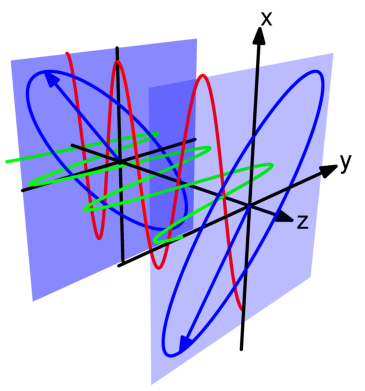
\includegraphics[height=0.2\textheight]{img/wellenplatte_eFeld.pdf}
                \caption[Rotation von Polarisationsellipsen]{Die Rotation von Polarisationsellipsen durch Halbwellenplatten. Rot und grün zeigen die Oszillation orthogonalen Komponenten des schwingenden elektrischen Feldes. Der elektrische Feldvektor wird in blau dargestellt. Der elektrische Feldvektor (blau) oszilliert mit der Zeit und folgt dabei der blauen Kurve. Der Polarisationszustand wird sowohl vor als auch nach dem Passieren der Halbwellenplatte gezeigt.}
                \label{fig:theo_wellenplatte_eFeld}
            \end{figure}
            
            Doppelbrechende Medien besitzen optische Achsen mit unterschiedlichem Brechungsindex. Dadurch durchlaufen zwei orthogonal stehende elektrische Felder den Stoff mit unterschiedlicher Geschwindigkeit und ihre Phasen werden gegeneinander verschoben~\cite{gil_polarized_2016}. Wellenplatten sind doppelbrechende Bauelemente, deren Dicke auf das Verhältnis ihrer Brechungsindices abgestimmt ist, um eine definierte Phasenverschiebung $\Delta$ zu erzeugen. Typisch sind Viertelwellenplatten ($\Delta=\nicefrac{\pi}{2}$), die zirkulare Polarisation in lineare Polarisation umwandeln, und Halbwellenplatten ($\Delta = \pi$), welche die Polarisationsellipse an der langsamen optischen Achse spiegeln~\cite{gil_polarized_2016}. Abbildung~\ref{fig:theo_wellenplatte_eFeld} illustriert diesen Effekt. Für linear polarisierte Strahlung ist die Spiegelung ununterscheidbar von einer Rotation um $2\varphi$, wenn $\varphi$ der Winkel zwischen der langsamen optischen Achse und der großen Ellipsenhalbachse ist. Folgende Matrix beschreibt die Polarisationseigenschaften einer idealen (vollständig transmittierenden) Halbwellenplatte~\cite{gil_polarized_2016}.
            \begin{equation*}
                \begin{pmatrix}
                    1 & 0 & 0 & 0 \\
                    0 & \cos(4\varphi) &  \sin(4\varphi) & 0 \\
                    0 & \sin(4\varphi) & -\cos(4\varphi) & 0 \\
                    0 & 0 & 0 & -1
                \end{pmatrix}
            \end{equation*}
            % General linear retarder
            %\begin{equation*}
            %    \resizebox{\hsize}{!}{$
            %        \begin{pmatrix}
            %            1 & 0 & 0 & 0 \\
            %            0 & \cos^2(2\varphi) + \cos(\Delta)\sin^2(2\varphi)   & [1-\cos(\Delta)]\sin(2\varphi)\cos(2\varphi)     & -\sin(2\varphi)\sin(\Delta) \\
            %           0 & [1-\cos(\Delta)]\sin(2\varphi)\cos(2\varphi)       & \sin^2(2\varphi) + \cos(\Delta)\cos^2(2\varphi) & \cos(2\varphi)\sin(\Delta) \\
            %            0 & \sin(2\varphi)\sin(\Delta)                        & -\cos(2\varphi)\sin(\Delta)                     &     \cos(\Delta)
            %        \end{pmatrix}
            %    $}
            %\end{equation*}
        
            Ein idealer Depolarisator überführt einen Stokesvektor in den vollständig unpolarisierten Stokesvektor $(1, 0, 0, 0)^T$ und erhält dabei die Intensität der Strahlung~\cite{gil_polarized_2016}. Wahre Depolarisation ist experimentell schwer zu erreichen. In der Praxis werden Geräte eingesetzt, die den Polarisationszustand zufällig mit der Zeit oder dem Ort variieren~\cite{wei_liquid_2016}. In vorliegender Arbeit wird ein Depolarisator aus Flüssigkristallpolymer eingesetzt. Dieser Bautyp besteht aus vielen unterschiedlich orientierten doppelbrechenden Domänen, die jede für sich wie eine Wellenplatte agieren. Durch Variation von Orientierung und Brechungsindices der optischen Achsen, wird die Polarisation randomisiert und die Strahlung verhält sich wie eine depolarisierte Welle~\cite{wei_liquid_2016}. Folgende Müllermatrix beschreibt den idealen Depolarisator~\cite{gil_polarized_2016}.
            \begin{equation*}
                \begin{pmatrix}
                    1 & 0 & 0 & 0 \\
                    0 & 0 & 0 & 0 \\
                    0 & 0 & 0 & 0 \\
                    0 & 0 & 0 & 0
                \end{pmatrix}
            \end{equation*}
        %
        %   RAMANSPETROMETER
        %
        \section{Aufbau und Anisotropie von Ramanspektrometern}\label{sec:theo_ramanspektrometer}
        
            
            
            Der Aufbau eines fasergekoppelten Ramanmikroskops ist in Abbildung~\ref{fig:theo_spektrometer} skizziert. Es besteht aus einem Laser als monochromatische Lichtquelle zur Anregung der Probe und einem Mikroskop, welches den Anregungslaser auf die Probe fokussiert. Gleichzeitig koppelt das Objektiv die rückgestreute Strahlung in das Spektrometer ein. Der Strahlenteiler ermöglicht das Beleuchten der Probe und Einfangen des Streulichts mit dem selben Objektiv. Ein Filter blockiert die Rayleighstreuung, sodass nur das Raman-gestreute Licht im Spektrometer analysiert wird. Das Spektrometer analysiert die Strahlung, indem ein optisches Gitter das einfallende Licht abhängig von seiner Wellenlänge auf unterschiedliche Pixel der CCD-Kamera streut.~\cite{muller_entwicklung_2017, delhaye_3_1996}
            
            \begin{figure}[!h]
                %
                %   Skizze Aufbau Ramanmikrospektrometer
                %
                \centering
                \subfloat[]{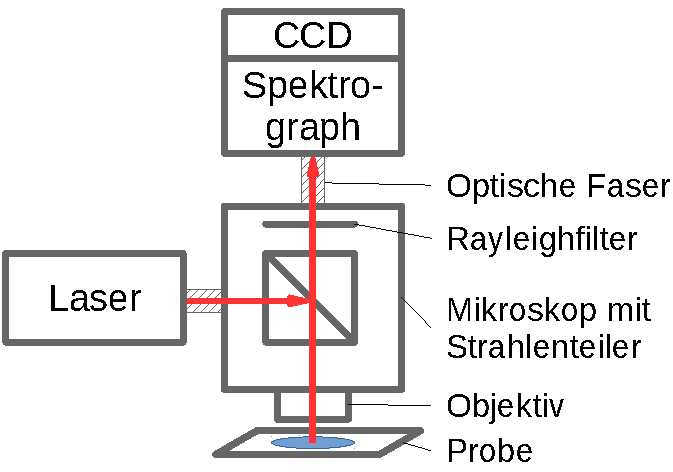
\includegraphics[height=0.3\textwidth]{img/spektrometer.pdf}\label{fig:theo_spektrometer}}
                \hfil
                \subfloat[]{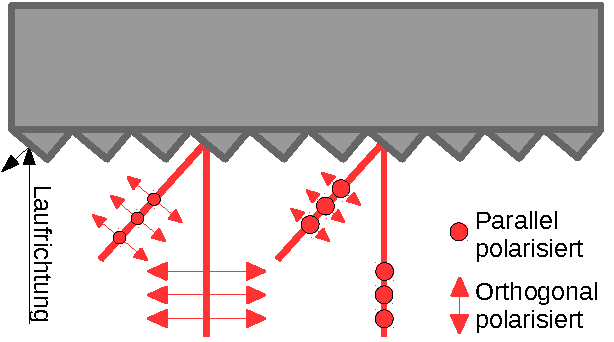
\includegraphics[width=0.5\textwidth]{img/polarisation_gitter.pdf}\label{fig:theo_gitter}}
                \caption[Skizze Ramanspektrometer]{\subref{fig:theo_spektrometer}~Aufbau eines fasergekoppelten Ramanmikroskops. \subref{fig:theo_gitter}~Streuung von polarisierter Strahlung ein einem Gitter. Orthogonal zum Gitter polarisierte Strahlung wird weniger gut als parallel polarisierte Strahlung.}
            \end{figure}
            
            Es ist bekannt, dass die Effizienz von Beugungsgittern von der Polarisation der gebeuten Lichtwelle abhängig ist ~\cite{kho_reduction_2005}. Typische Gitter, die in der Spektroskopie Anwendung finden, beugen das Licht aufgrund einer eindimensionalen Gitterstruktur auf ihrer Oberfläche (Abb.~\ref{fig:theo_gitter}). Ob das Licht parallel oder orthogonal zu den Gitterfurchen polarisiert ist, beeinflusst die Beugung der Lichtwelle am Gitter~\cite{kho_reduction_2005}. Folglich kann ein zufällig fluktuierender oder unbekannter Polarisationszustand die Vergleichbarkeit von Ramanspektrometern beeinträchtigen~\cite{kho_reduction_2005}.
            
        %
        %   OPTISCHE FASERN
        %
        \section{Aufbau und Funktionsweise optischer Fasern}
            
            In einem nicht absorbierenden zylindrischen Stab, dessen Brechungsindex größer ist als die der des umgebenden Mediums, können Lichtstrahlen durch Totalreflexion an das andere Ende geleitet werden. Ein solche optische Faser oder auch Wellenleiter besteht häufig aus einem Kern aus Glas und einem Mantel aus dotiertem Glas~\cite{pedrotti_optik_2005}. Abbildung~\ref{fig:theo_lichtwellenleiter} skizziert die Kopplung eines Strahls in die Faser und seine Reflexion in der Faser. Trifft ein Lichtstrahl im Winkel $\varepsilon$ auf die Stirnfläche der Faser wird er gebrochen und trifft in der Faser mit dem Winkel $\varepsilon^\prime$ auf die Kern-Mantel-Grenze. Wenn der Winkel $\nicefrac{\pi}{2} - \varepsilon^\prime$ größer oder gleich dem Grenzwinkel für Totalreflexion $\gamma$ ist, breitet sich das Licht ohne Reflexionsverluste in der Faser aus~\cite{pedrotti_optik_2005}. Ist $\nicefrac{\pi}{2} - \varepsilon^\prime$ kleiner als $\gamma$ transmittiert ein Teil der Strahlung die Kern-Mantel-Grenze und verlässt die Faser: Es kommt zu Intensitätsverlusten. Weil der Lichtstrahl sehr oft in der Faser reflektiert wird, haben die Reflexionsverluste einen großen Einfluss auf die Lichtleitung~\cite{pedrotti_optik_2005}. Der Winkel $2\varepsilon$ ist der Akzeptanzwinkel der Faser. Je größer er ist, desto mehr Licht kann in die Faser eingekoppelt werden~\cite{pedrotti_optik_2005}.
            
            Die Biegung von optischen Fasern oder Mikrodefekte in ihrer Oberfläche ändern den Winkel $\varepsilon^\prime$. Werden dadurch die Bedingungen der Totalreflexion verletzt werden, treten Reflexionsverluste auf~\cite{pedrotti_optik_2005}.
            
            \begin{figure}[!b]
                \centering
                \subfloat[]{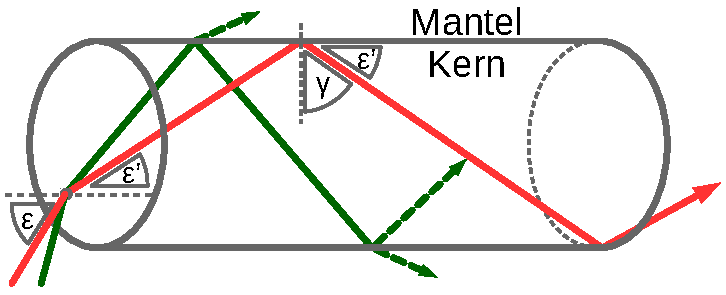
\includegraphics[width=0.49\textwidth]{img/lichtwellenleiter.pdf}
                \label{fig:theo_lichtwellenleiter}}
                \subfloat[]{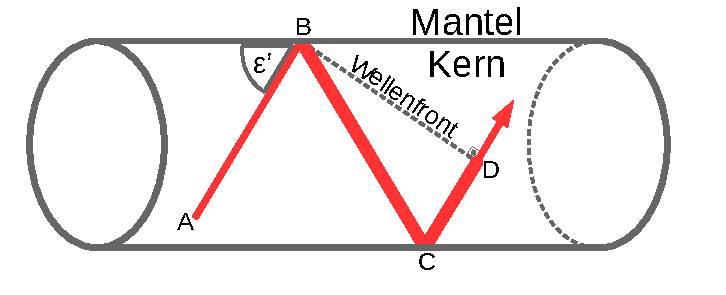
\includegraphics[width=0.49\textwidth]{img/lichtwellenleiter_moden.pdf}
                \label{fig:theo_lichtwellenleiter_moden}}
                \caption[Lichtleitung in optischen Fasern]{\subref{fig:theo_lichtwellenleiter}~Lichtstrahlen werden in optischen Fasern durch Totalreflexion an der Faserkern-Mantel-Grenze geleitet (rot). Fällt das Licht zu steil auf die Stirnfläche, findet keine Totalreflexion statt und die Intensität der geleiteten Welle nimmt schnell ab (grün)~\cite{pedrotti_optik_2005}. \subref{fig:theo_lichtwellenleiter_moden}~Nicht jede Schwingungsmode ist in optischen Fasern erlaubt. Verschiebt die Reflexion bei $B$ und $C$ die Phasen der Teilstrahlen $\overline{AB}$ und $\overline{CD}$, sodass die Phasen entlang de Wellenfront $\overline{BD}$ übereinstimmen, interferieren sie konstruktiv~\cite{pedrotti_optik_2005}.}
            \end{figure}
            
            Lichtstrahlen müssen eine weitere Bedingung erfüllen, um durch die Faser geleitet werden zu können. Abbildung~\ref{fig:theo_lichtwellenleiter_moden} zeigt den Weg eines Lichtstrahls durch eine Faser, der an den Punkten $B$ und $C$ totalreflektiert wird. Die Doppelreflexion führt zu einer Phasenverschiebung der Teilstrahlen $\overline{AB}$ und $\overline{CD}$, die abhängig vom Einfallswinkel $\varepsilon^\prime$ ist. Es können sich nur Wellen in der Faser ausbreiten, deren Phasen entlang der Wellenfront $\overline{BD}$ übereinstimmen und konstruktiv interferieren~\cite{pedrotti_optik_2005}. Eine solche Welle ist eine erlaubte Schwingungsmode~\cite{pedrotti_optik_2005}.
            
            Mikrodefekte in der Faser haben Auswirkungen auf die Schwingungsmoden. Verformungen der Kern-Mantel-Grenze ändern lokal den Einfallswinkel $\varepsilon^\prime$ und können dadurch Energie in eine andere Mode pumpen. Die Moden sind gekoppelt~\cite{pedrotti_optik_2005}.
            
            Fasern mit großem Kerndurchmesser besitzen viele erlaubte Moden und werden als Mehrmodenfaser, Multi-mode Faser oder MM-Faser bezeichnet~\cite{pedrotti_optik_2005}. Der Kerndurchmesser von Einmodenfasern ist hinreichend klein, sodass sich nur eine Mode ausbreiten kann~\cite{pedrotti_optik_2005}. Einmodenfasern werden auch Single-mode Faser oder SM-Faser genannt. Diese besitzen einen so kleinen Kerndurchmesser, dass sich ihr Verhalten nicht alleine durch Strahlenoptik erklären lässt. Aufgrund des kleinen Kerns wird Licht vermehrt als evaneszente Welle im Fasermantel geleitet~\cite{pedrotti_optik_2005}. Evaneszenz beschreibt das Phänomen, dass totalreflektierte Felder an der Kern-Mantel-Grenze nicht verschwinden. Die Amplitude des elektrischen Feldes nimmt im Mantel exponentiell ab und ein Teil der Strahlung wird als evaneszente Welle geleitet~\cite{pedrotti_optik_2005}. Weil Einmodenfasern mehr als ein Drittel des Lichts im Mantel leiten können, sind sie empfindlicher gegenüber dem Biegen der Faser oder Mikrodefekten im Mantel~\cite{pedrotti_optik_2005}. 
            
            Ideale optische Fasern sind radial symmetrisch und besitzen einen isotropen Kern. Dadurch kann die Polarisation von elektromagnetischen Wellen, wie in den vorherigen Überlegungen, durch zwei orthogonale oszillierende elektrische Felder beschrieben werden. Durch den isotropen Kern bleibt ihre Phasenbeziehung konstant und beliebige Polarisationszustände werden erhalten~\cite{ma_characterization_2009}. Reale Fasern sind nicht perfekt zylindrisch und zeigen durch mechanischen Stress lokal Doppelbrechung. Der mechanische Stress kann durch temperaturbedingte Materialdehnung, Krümmung oder Verdrehen der Faser entstehen. Besitzt nun eine Faser mehrere anisotrope Zentren mit unterschiedlich orientierten optischen Achsen, wird die Phasenbeziehung der elektrischen Felder randomisiert und das Licht depolarisiert~\cite{ma_characterization_2009}.
            
            Polarisationserhaltende Fasern (PM-Fasern) werden mit einem anisotropen Kern gefertigt. Die Brechungszahlen der gewollten optischen Achsen unterscheiden sich dabei mehr als die lokalen doppelbrechenden Zentren, die auch in PM-Fasern stressbedingt entstehen können. Dadurch wird die Kopplung der Polarisationsmoden verhindert und die Faser erhält lineare Polarisationszustände, die parallel zu den optischen Achsen polarisiert sind~\cite{ma_characterization_2009}. Alle anderen Polarisationszustände werden nicht erhalten. Wie bei einer Wellenplatte laufen die Polarisationsmoden unterschiedlich schnell durch die Faser und werden gegeneinander phasenverschoben: Es entsteht elliptisch polarisierte Strahlung~\cite{ma_characterization_2009}. Aufgrund des großen Brechungsindexunterschiedes der optischen Achsen ist die Modenkopplung, die stattfindet, vermutlich sehr ineffizient und bedingt Intensitätsverluste. Allgemein sind polarisationsabhängige Intensitätsverluste (polarisation dependent loss, PDL) ein bekanntes Problem in der Faseroptik~\cite{ping_lu_statistical_2001, mecozzi_statistics_2002}.
            

\end{document}